\documentclass[tikz,border=10pt]{standalone}
\usetikzlibrary{arrows.meta, patterns}
\begin{document}
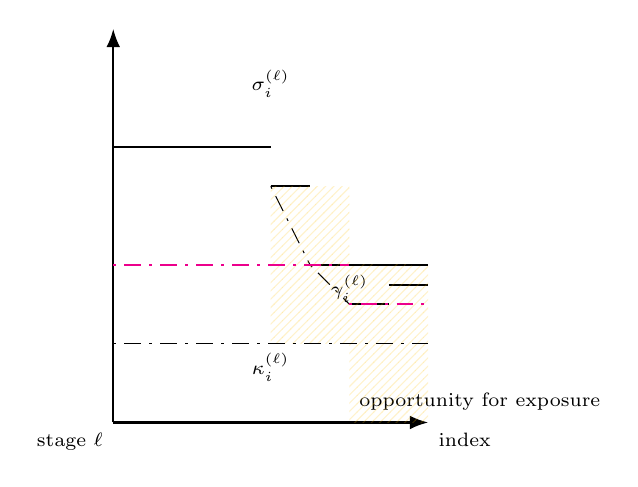
\begin{tikzpicture}[
    xscale=4, yscale=2,
    every node/.style={font=\scriptsize},
    axis/.style={black, thick, -Latex},
    important line/.style={thick},
    dashed line/.style={dash pattern=on 1pt off 3pt on 6pt off 3pt},
    opportunity/.style={pattern=north east lines, pattern color=orange!50!yellow},
]

% Draw axis
\draw[axis] (0,0) node[below left] {stage $\ell$} -- (0,2.5);
\draw[axis] (0,0) -- (1,0) node[below right] {index};

% Labels
\node[above] at (0.5,2) {$\sigma_i^{(\ell)}$};
\node[below] at (0.5,0.5) {$\kappa_i^{(\ell)}$};
\node[below right] at (0.75,0.25) {opportunity for exposure};
\node[below] at (0.75,1) {$\gamma_i^{(\ell)}$};

% Draw lines
\draw[important line] (0,1.75) -- (0.5,1.75);
\draw[important line] (0.5,1.5) -- (0.625,1.5);
\draw[important line] (0.625,1) -- (0.75,1);
\draw[dashed line] (0.5,1.5) -- (0.625,1);
\draw[dashed line] (0.625,1) -- (0.75,0.75);
\draw[important line] (0.75,1) -- (1,1);
\draw[important line] (0.75,0.75) -- (0.875,0.75);
\draw[important line] (0.875,0.875) -- (1,0.875);

% Draw shaded areas
\fill[opportunity, opacity=0.2] (0.5,0.5) rectangle (0.75,1.5);
\fill[opportunity, opacity=0.2] (0.75,0) rectangle (1,1);

% Draw dashed lines for $\kappa_i^{(\ell)}$ and $\gamma_i^{(\ell)}$
\draw[dashed line] (0,0.5) -- (1,0.5);
\draw[dashed line] (0,1) -- (1,1);
\draw[magenta, dashed line, thick] (0,1) -- (0.75,1);
\draw[magenta, dashed line, thick] (0.75,0.75) -- (1,0.75);

\end{tikzpicture}
\end{document}